\documentclass[a4paper,11pt]{article}

\usepackage[english]{babel}
\usepackage[utf8]{inputenc}
\usepackage[vmargin=3.5cm,hmargin=2cm]{geometry}
\usepackage{graphicx}
\usepackage{caption}
\usepackage{subcaption}
\usepackage{amsmath}
\usepackage{mathtools}
\usepackage{fancyhdr}

\setlength{\footskip}{0cm}
\setlength\parindent{0pt} %Quita la sangría francesa
\addtolength{\footskip}{0.8cm}
\addtolength{\headsep}{-.5cm}

\title{\bfseries Report:\\}
\date{}

\lfoot{}
\cfoot{}
\rfoot{\textbf{Signal Theory} \\ Teresa Algarra Ulierte }

\renewcommand{\headrulewidth}{0.5pt}
\renewcommand{\footrulewidth}{0.5pt}

\begin{document}
\renewcommand\contentsname{\vspace{-1cm}}
\maketitle

\begin{centering}
    Teresa Algarra Ulierte \\
    Student ID: teral436 \\
    Personnummer: 970628T129 \\
\end{centering}

\vspace{1cm}

\begin{figure}[!ht]
	\centering
	
\includegraphics[scale = 0.5]{images/portada.jpeg}
\end{figure}

\newpage

\section{Study 1: Modelling Signals}

%%%THEORETICAL BACKGROUND%%%

\subsection{Theoretical Background:}

In this study we will work with white noise, which is defined as a process with constant PSD.

\begin{equation}R_0 = \frac{N_0}{2}\end{equation}

It is also known that the white noise is Gaussian, which means that if it is WSS, it will be SSS. As we want it to be scalled, we will use $R_x=1$.

So first we have the noise:

\begin{figure}[!hp]
\centering
\begin{minipage}{.5\textwidth}
  \centering
  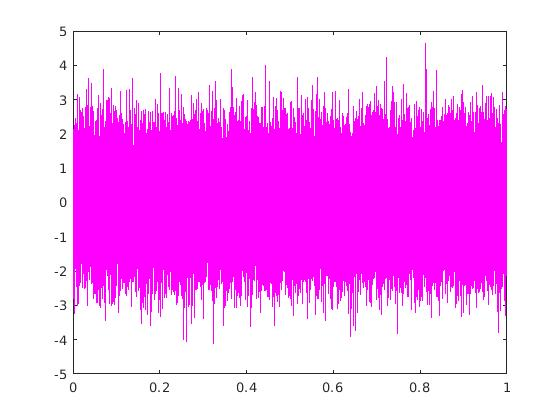
\includegraphics[width=1\linewidth]{images/lab1_1.jpg}
  \captionof{figure}{Noise}
\end{minipage}%
\begin{minipage}{.5\textwidth}
  \centering
  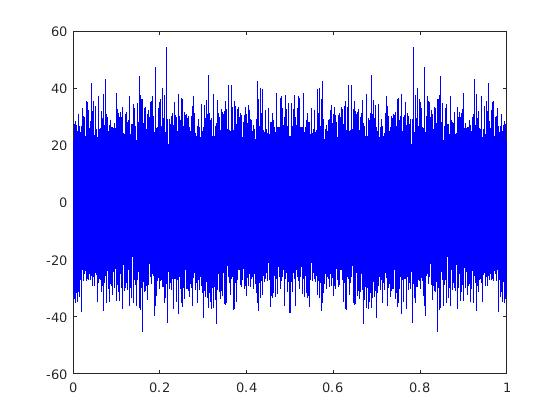
\includegraphics[width=1\linewidth]{images/lab1_2.jpg}
  \captionof{figure}{Noise in frequency domain}
\end{minipage}
\end{figure}

We will get this noise through some LTI filters, having:

\begin{equation}R_y(f) = R_x |H(f)|^2\end{equation}

\newpage

%%%THEORETICAL ANALYSIS%%%

\subsection{Theoretical Analysis:}

To get to calculate the ACF and the PSD of the result function, we have to know exactly what filters we are using.

For the ideal filter, we can use the rectangle function:

\begin{equation}H[\theta] = rect(\frac{\theta}{\theta_0})\end{equation}

\begin{figure}[!hp]
\centering
\begin{minipage}{.5\textwidth}
  \centering
  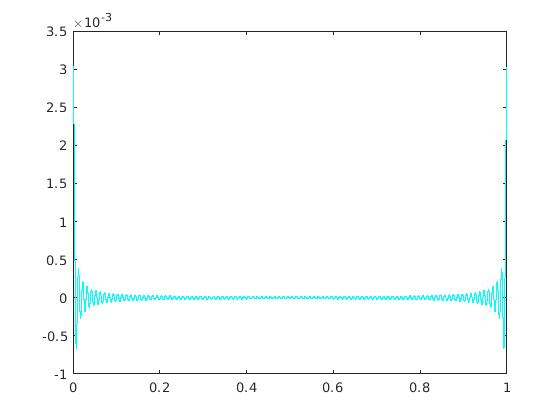
\includegraphics[width=1\linewidth]{images/lab1_5.jpg}
  \captionof{figure}{Filter in time domain}
\end{minipage}%
\begin{minipage}{.5\textwidth}
  \centering
  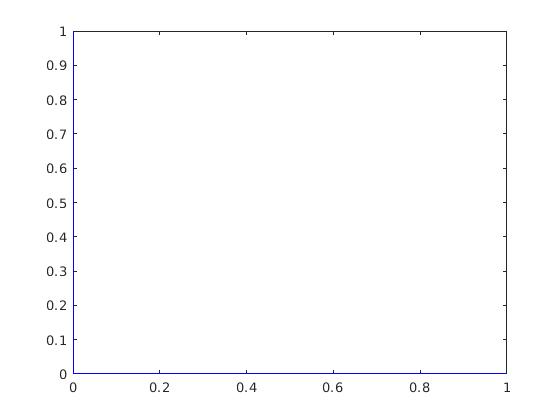
\includegraphics[width=1\linewidth]{images/lab1_4.jpg}
  \captionof{figure}{Filter frequency domain}
\end{minipage}
\end{figure}

The filtered signal is:

\begin{figure}[!hp]
\centering
\begin{minipage}{.5\textwidth}
  \centering
  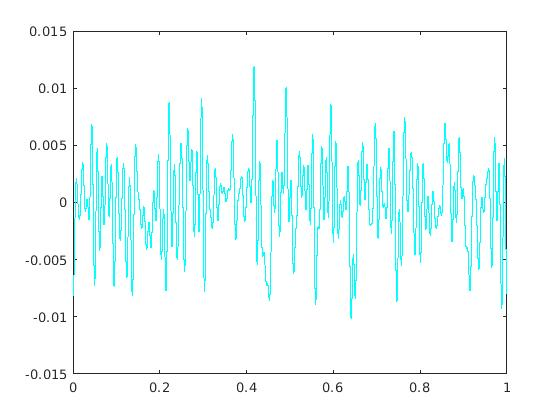
\includegraphics[width=1\linewidth]{images/lab1_8.jpg}
  \captionof{figure}{Filtered signal}
\end{minipage}%
\begin{minipage}{.5\textwidth}
  \centering
  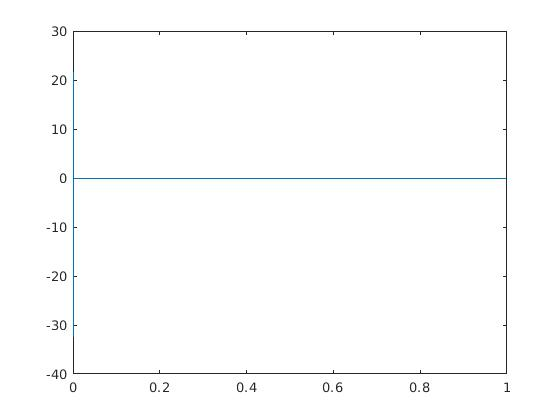
\includegraphics[width=1\linewidth]{images/lab1_6.jpg}
  \captionof{figure}{Filtered signal in frequency domain}
\end{minipage}
\end{figure}

\newpage

For the low-degree low-pass filter, we will use a first-order Butterworth filter:

\begin{equation}H(z) = \frac{b}{a_1-a_2e^{-j2 \pi f}}\end{equation}

We will use $b = a_1 = 1$ and $a_2 = 0.9$.

\begin{figure}[!hp]
\centering
\begin{minipage}{.5\textwidth}
  \centering
  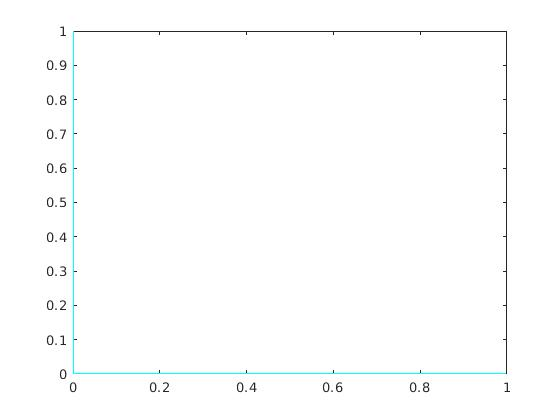
\includegraphics[width=1\linewidth]{images/lab1_25.jpg}
  \captionof{figure}{Filter}
\end{minipage}%
\begin{minipage}{.5\textwidth}
  \centering
  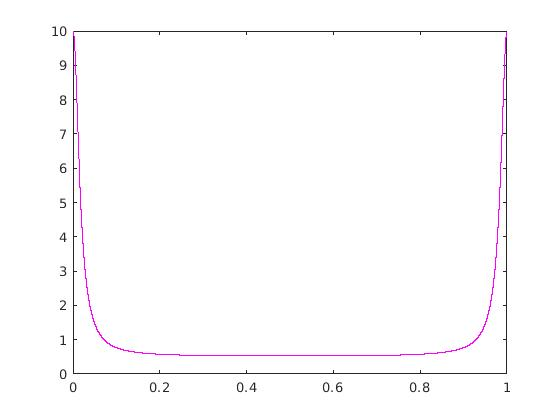
\includegraphics[width=1\linewidth]{images/lab1_23.jpg}
  \captionof{figure}{Filter in frequency domain}
\end{minipage}
\end{figure}

The filtered signal is:

\begin{figure}[!hp]
\centering
\begin{minipage}{.5\textwidth}
  \centering
  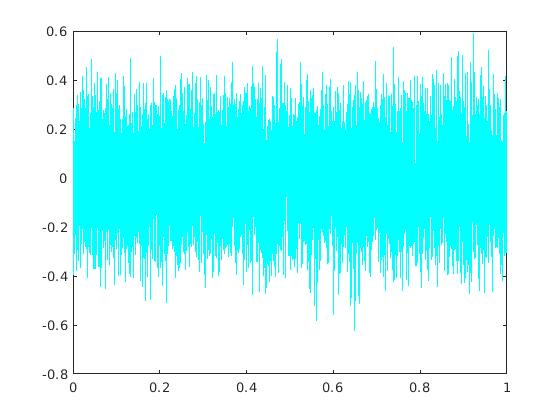
\includegraphics[width=1\linewidth]{images/lab1_28.jpg}
  \captionof{figure}{Filtered signal}
\end{minipage}%
\begin{minipage}{.5\textwidth}
  \centering
  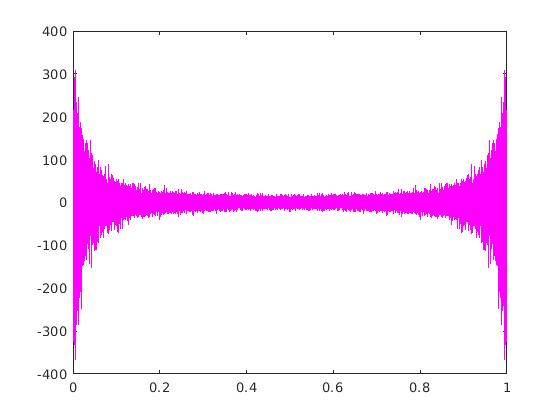
\includegraphics[width=1\linewidth]{images/lab1_26.jpg}
  \captionof{figure}{Filtered signal in frequency domain}
\end{minipage}
\end{figure}

\newpage

So, we can start by calculating the theoretical PSD knowing the super-formula:

\begin{equation}R_y[\theta] = R_x|H(\theta)|^2\end{equation}

As we are working with White Gaussian Noise, its PSD it's going to be $\frac{N_0}{2}$ as said before, therefore we have:

\begin{equation}R_y[\theta] = \frac{N_0}{2}|H(\theta)|^2\end{equation}

For the ideal filter, the result is:

\begin{equation}R_y[\theta] = \frac{N_0}{2}|rect(\frac{\theta}{\theta_0})|^2 = \frac{N_0}{2}rect(\frac{\theta}{\theta_0}) = \frac{N_0}{2} if \theta < \theta_0 \end{equation}

For the low-degree filter, the result is:

\begin{equation}R_y[\theta] = \frac{N_0}{2}|\frac{b}{a_1-a_2e^{-j2 \pi f}}|^2 = \frac{N_0}{2|1-0.9e^{-j2 \pi f}|^2} \end{equation}

Let's get on to the graphs.

\newpage

\subsubsection{Ideal filter:}

We get the following ACF:

\begin{figure}[!hp]
\centering
\begin{minipage}{.5\textwidth}
  \centering
  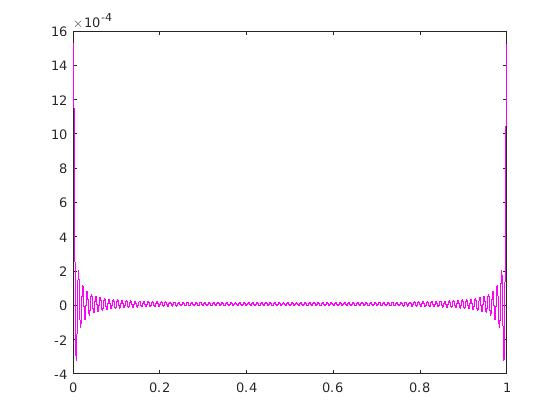
\includegraphics[width=1\linewidth]{images/lab1_9.jpg}
  \captionof{figure}{Theoretical ACF plotted}
\end{minipage}%
\begin{minipage}{.5\textwidth}
  \centering
  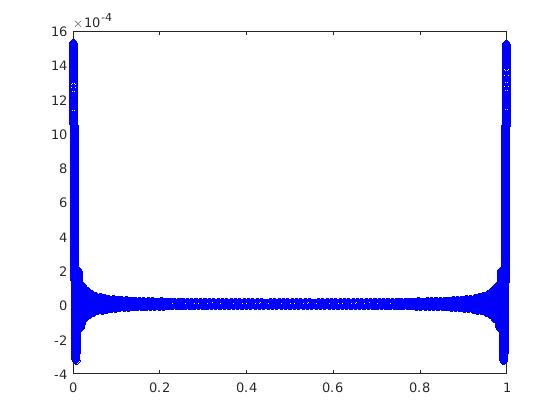
\includegraphics[width=1\linewidth]{images/lab1_10.jpg}
  \captionof{figure}{Theoretical ACF stemed}
\end{minipage}
\end{figure}

We get the following PSD:

\begin{figure}[!hp]
    \begin{center}
      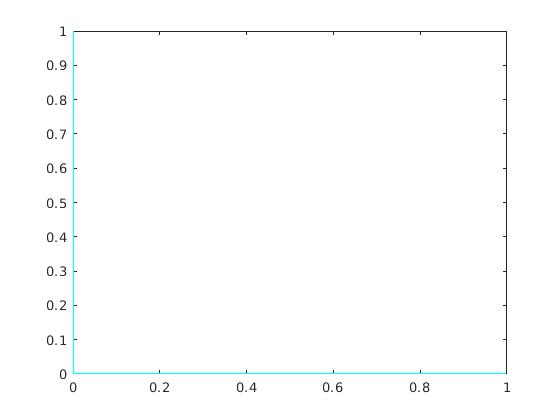
\includegraphics[width=0.6\textwidth]{images/lab1_15.jpg}
      \captionof{figure}{Theoretical PSD}
    \end{center}
\end{figure}

\newpage

\subsubsection{Low-degree filter:}

We get the following ACF:

\begin{figure}[!hp]
\centering
\begin{minipage}{.5\textwidth}
  \centering
  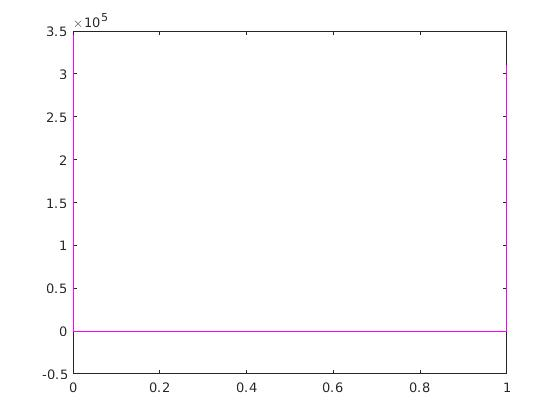
\includegraphics[width=1\linewidth]{images/lab1_29.jpg}
  \captionof{figure}{Theoretical ACF plotted}
\end{minipage}%
\begin{minipage}{.5\textwidth}
  \centering
  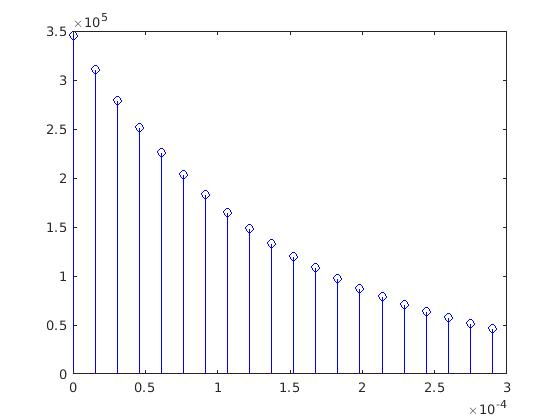
\includegraphics[width=1\linewidth]{images/lab1_30.jpg}
  \captionof{figure}{Theoretical ACF stemed}
\end{minipage}
\end{figure}

We get the following PSD:

\begin{figure}[!hp]
    \begin{center}
      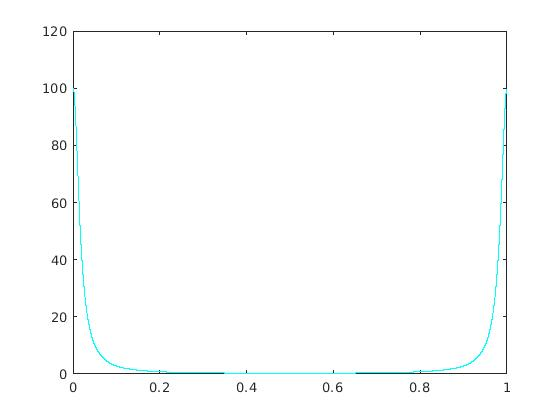
\includegraphics[width=0.6\textwidth]{images/lab1_35.jpg}
      \captionof{figure}{Theoretical PSD}
    \end{center}
\end{figure}

\newpage

\subsection{Estimations:}

\subsubsection{Ideal filter}

For the ideal filter, we will use a tenth order butterworth filter.

We get the following PSD:

\begin{figure}[!hp]
    \begin{center}
      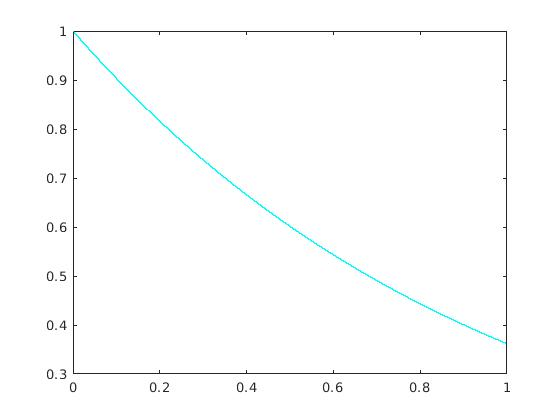
\includegraphics[width=0.6\textwidth]{images/lab1_22.jpg}
      \captionof{figure}{Estimated PSD}
    \end{center}
\end{figure}

If we estimate by the Bartlett method, we get the following ACF:

\begin{figure}[!hp]
\centering
\begin{minipage}{.5\textwidth}
  \centering
  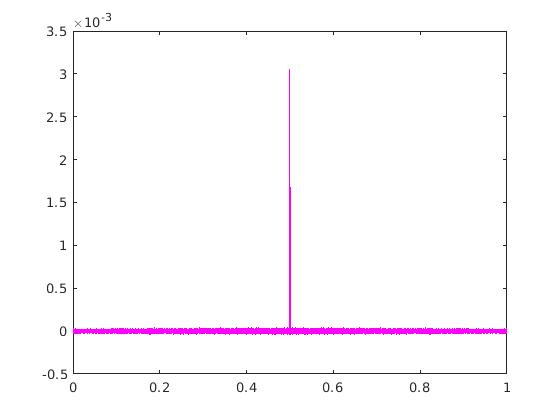
\includegraphics[width=1\linewidth]{images/lab1_18.jpg}
  \captionof{figure}{Estimated by Bartlett ACF plotted}
\end{minipage}%
\begin{minipage}{.5\textwidth}
  \centering
  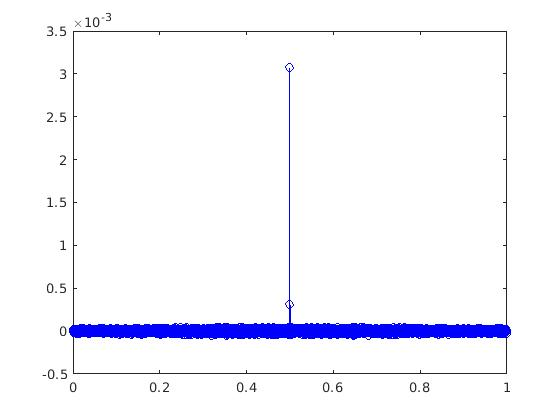
\includegraphics[width=1\linewidth]{images/lab1_19.jpg}
  \captionof{figure}{Estimated by Bartlett ACF stemed}
\end{minipage}
\end{figure}

\newpage

If we estimate by the Blackman-Harris method, we get the following ACF:

\begin{figure}[!hp]
\centering
\begin{minipage}{.5\textwidth}
  \centering
  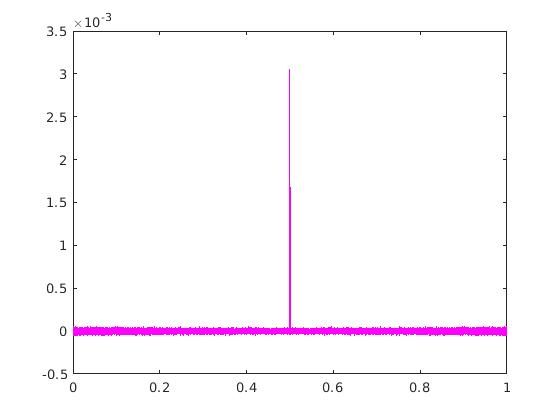
\includegraphics[width=1\linewidth]{images/lab1_20.jpg}
  \captionof{figure}{Estimated by Blackman-Harris ACF plotted}
\end{minipage}%
\begin{minipage}{.5\textwidth}
  \centering
  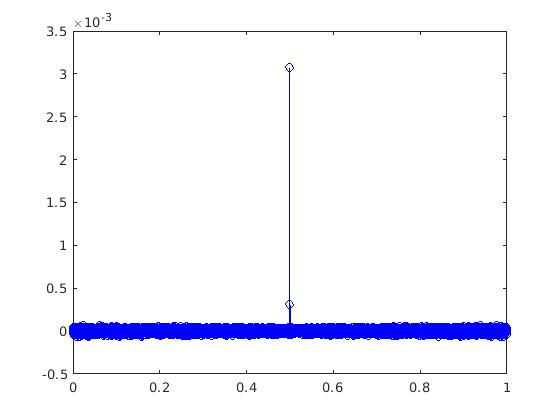
\includegraphics[width=1\linewidth]{images/lab1_21.jpg}
  \captionof{figure}{Estimated by Blackman-Harris ACF stemed}
\end{minipage}
\end{figure}

\subsubsection{Low-degree filter}

For the low-degree filter, we will use a first order butterworth filter.

We get the following PSD:

\begin{figure}[!hp]
    \begin{center}
      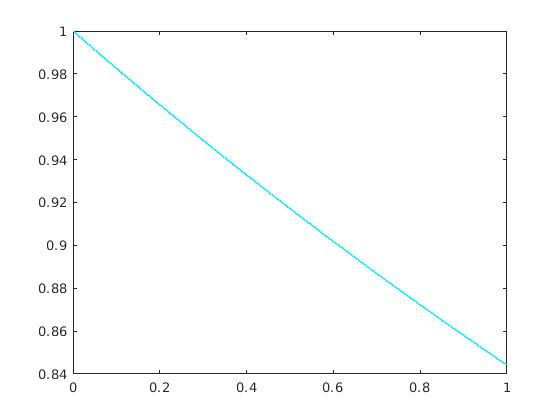
\includegraphics[width=0.6\textwidth]{images/lab1_42.jpg}
      \captionof{figure}{Estimated PSD}
    \end{center}
\end{figure}

\newpage

If we estimate by the Bartlett method, we get the following ACF:

\begin{figure}[!hp]
\centering
\begin{minipage}{.5\textwidth}
  \centering
  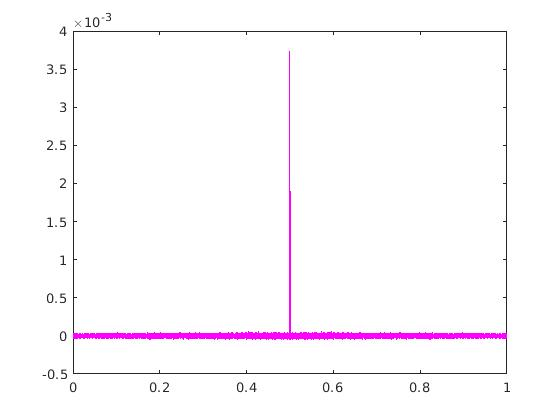
\includegraphics[width=1\linewidth]{images/lab1_38.jpg}
  \captionof{figure}{Estimated by Bartlett ACF plotted}
\end{minipage}%
\begin{minipage}{.5\textwidth}
  \centering
  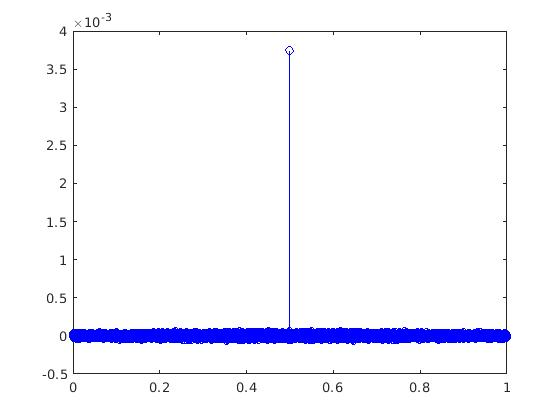
\includegraphics[width=1\linewidth]{images/lab1_39.jpg}
  \captionof{figure}{Estimated by Bartlett ACF stemed}
\end{minipage}
\end{figure}

If we estimate by the Blackman-Harris method, we get the following ACF:

\begin{figure}[!hp]
\centering
\begin{minipage}{.5\textwidth}
  \centering
  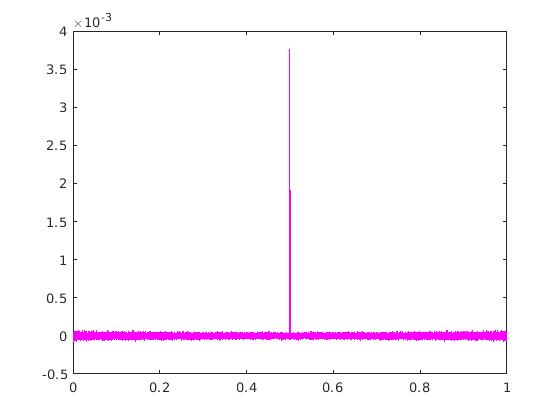
\includegraphics[width=1\linewidth]{images/lab1_40.jpg}
  \captionof{figure}{Estimated by Blackman-Harris ACF plotted}
\end{minipage}%
\begin{minipage}{.5\textwidth}
  \centering
  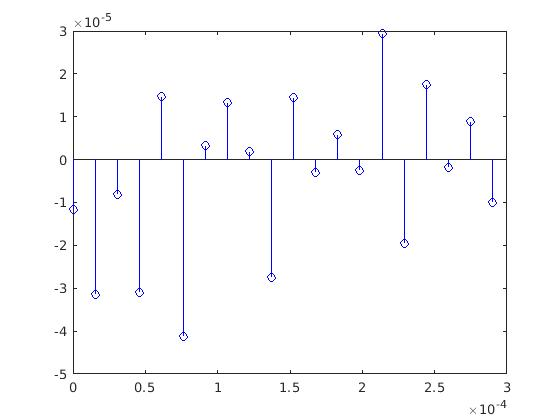
\includegraphics[width=1\linewidth]{images/lab1_41.jpg}
  \captionof{figure}{Estimated by Blackman-Harris ACF stemed}
\end{minipage}
\end{figure}

\newpage

\subsection{Final Comparation:}

\begin{itemize}

\item Ideal filter:

As we can see, the changes from the ideal filter to a tenth order filter are really big. Maybe it would have been more accurate to pick a 15th order filter, or something even bigger. The PSD goes from being a step to being a curve, and the ACF goes from having a peak in 0 to having it in 0.5, so the changes are bigger than desirable.
There is not a big difference between the Bartlett estimation and the Blackman-Harris one.

\item Low-degree filter:

The changes from this filter to the estimated one are also really big. The PSD is not as expected, and more than a curve it's almost a down-going straight line. The ACF has the same problem as the ideal filter, the peak has been moved to 0.5 in stead of 0.

\end{itemize}

\newpage

\section{Study 2:}

\subsection{Theoretical Background:}

In this second study, the aim is to improve the estimates done in the first study.
We will use the same White Gaussian noise and both filters.
In order to improve our estimations, we will use \textit{windows}, in which case we have a few possibilities,
of which we will explore:

\begin{itemize}
  \item \textit{Rectangular window}
  \item \textit{Triangle window}.
  \item \textit{Hamming window}.
  \item \textit{Bartlett window}
  \item \textit{Blackman-Harris window}.
\end{itemize}

Here we show the different windows used:

\begin{figure}[!hp]
\centering
\begin{minipage}{.5\textwidth}
  \centering
  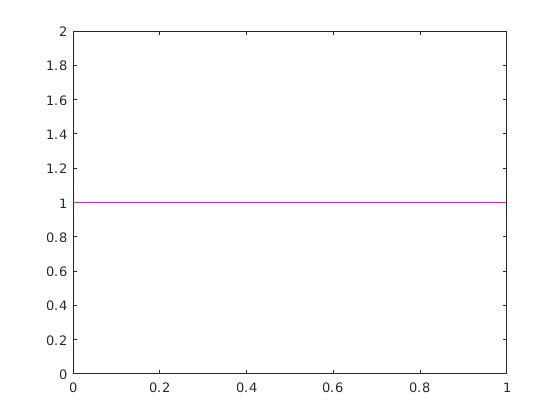
\includegraphics[width=1\linewidth]{images/lab2_1.jpg}
  \captionof{figure}{Rectangular window}
\end{minipage}%
\begin{minipage}{.5\textwidth}
  \centering
  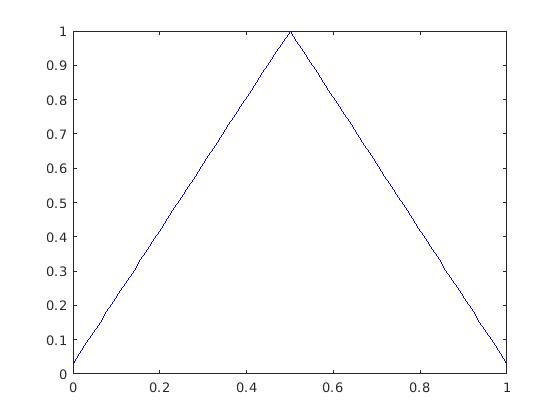
\includegraphics[width=1\linewidth]{images/lab2_2.jpg}
  \captionof{figure}{Triangular window}
\end{minipage}
\end{figure}

\newpage

\begin{figure}[!hp]
\centering
\begin{minipage}{.5\textwidth}
  \centering
  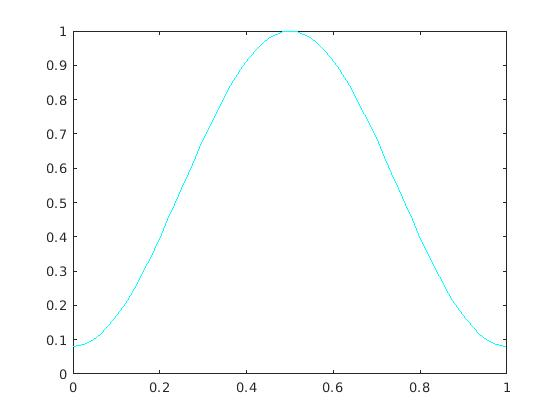
\includegraphics[width=1\linewidth]{images/lab2_3.jpg}
  \captionof{figure}{Hamming window}
\end{minipage}%
\begin{minipage}{.5\textwidth}
  \centering
  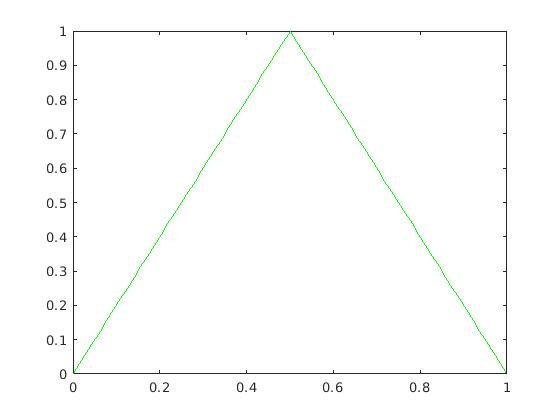
\includegraphics[width=1\linewidth]{images/lab2_4.jpg}
  \captionof{figure}{Bartlett window}
\end{minipage}
\end{figure}

\begin{figure}[!hp]
    \begin{center}
      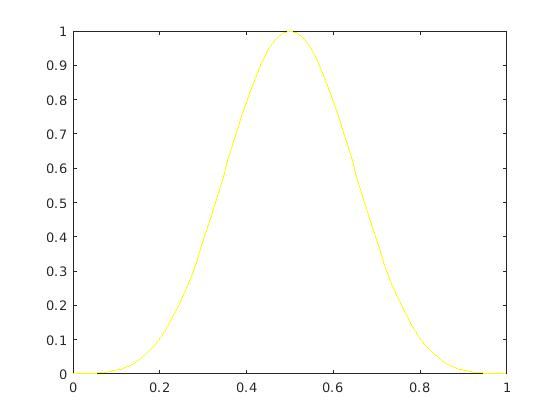
\includegraphics[width=0.6\textwidth]{images/lab2_5.jpg}
      \captionof{figure}{Blackman-Harris window}
    \end{center}
\end{figure}

\newpage

\subsection{Improved Estimates: Ideal filter}

For this section we will take the estimations done during the first study with the tenth degree Butterworth filter.

We have the following PSD:

\begin{figure}[!hp]
    \begin{center}
      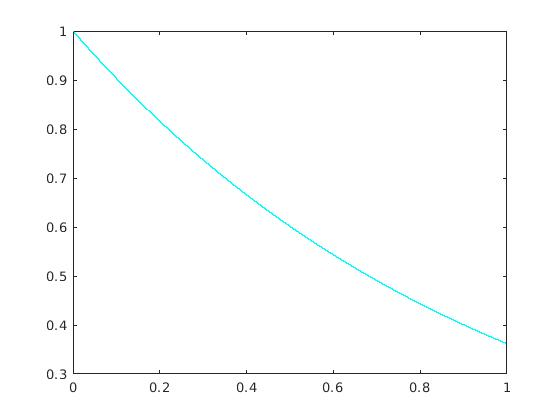
\includegraphics[width=0.6\textwidth]{images/lab2_12.jpg}
      \captionof{figure}{Estimated PSD}
    \end{center}
\end{figure}

If we estimate by the Bartlett method, we get the following ACF:

\begin{figure}[!hp]
\centering
\begin{minipage}{.5\textwidth}
  \centering
  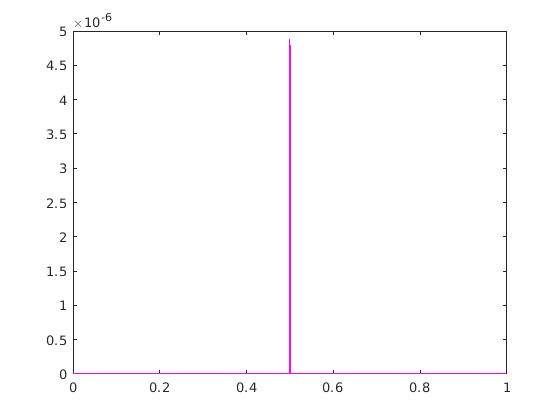
\includegraphics[width=1\linewidth]{images/lab2_8.jpg}
  \captionof{figure}{Estimated by Bartlett ACF plotted}
\end{minipage}%
\begin{minipage}{.5\textwidth}
  \centering
  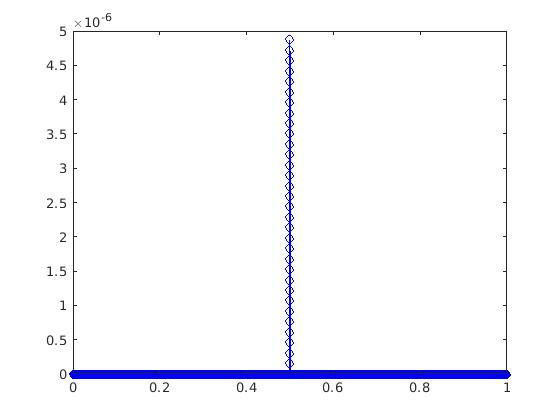
\includegraphics[width=1\linewidth]{images/lab2_9.jpg}
  \captionof{figure}{Estimated by Bartlett ACF stemed}
\end{minipage}
\end{figure}

\newpage

If we estimate by the Blackman-Harris method, we get the following ACF:

\begin{figure}[!hp]
\centering
\begin{minipage}{.5\textwidth}
  \centering
  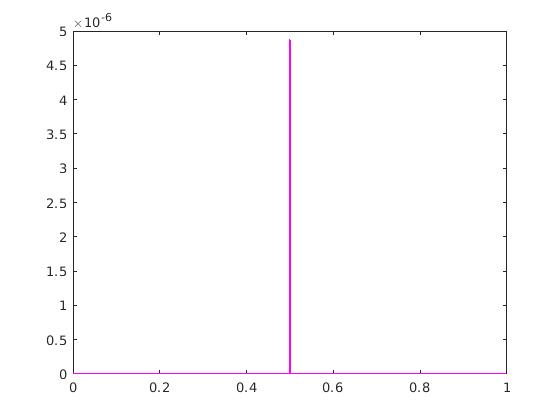
\includegraphics[width=1\linewidth]{images/lab2_10.jpg}
  \captionof{figure}{Estimated by Blackman-Harris ACF plotted}
\end{minipage}%
\begin{minipage}{.5\textwidth}
  \centering
  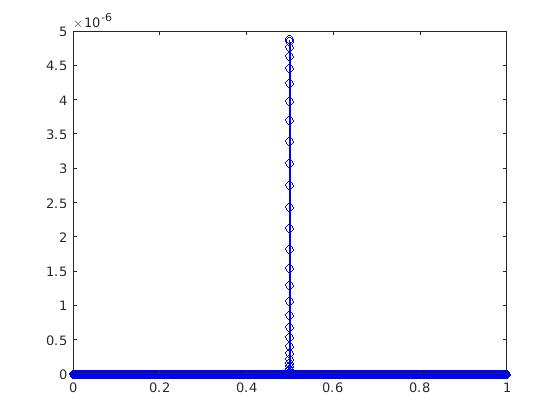
\includegraphics[width=1\linewidth]{images/lab2_11.jpg}
  \captionof{figure}{Estimated by Blackman-Harris ACF stemed}
\end{minipage}
\end{figure}

\subsubsection{Rectangular Window:}

Here we will get our filtered signal by a filter which is our rectangular window. There are the results:

\begin{figure}[!hp]
    \begin{center}
      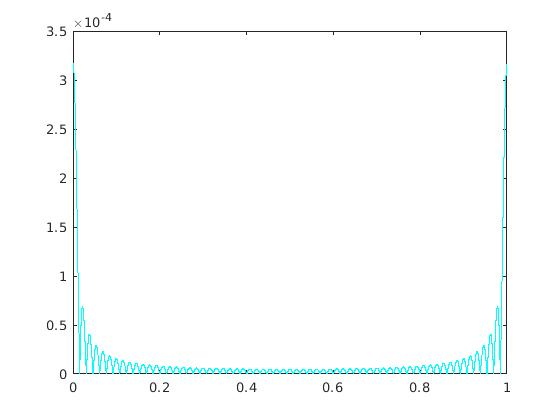
\includegraphics[width=0.6\textwidth]{images/lab2_19.jpg}
      \captionof{figure}{Improved PSD}
    \end{center}
\end{figure}

\newpage

\begin{figure}[!hp]
\centering
\begin{minipage}{.5\textwidth}
  \centering
  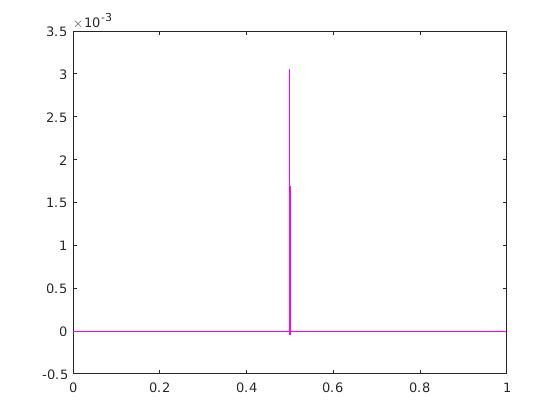
\includegraphics[width=1\linewidth]{images/lab2_15.jpg}
  \captionof{figure}{Improved ACF plotted (Bartlett)}
\end{minipage}%
\begin{minipage}{.5\textwidth}
  \centering
  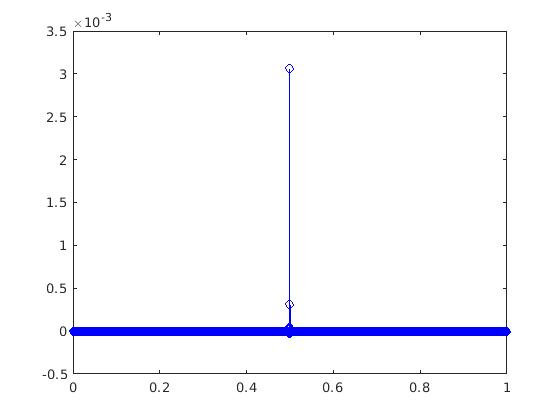
\includegraphics[width=1\linewidth]{images/lab2_16.jpg}
  \captionof{figure}{Improved ACF stemed (Bartlett)}
\end{minipage}
\end{figure}

\begin{figure}[!hp]
\centering
\begin{minipage}{.5\textwidth}
  \centering
  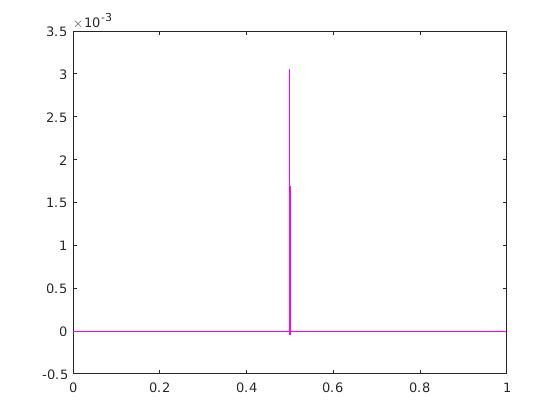
\includegraphics[width=1\linewidth]{images/lab2_17.jpg}
  \captionof{figure}{Improved ACF plotted (Blackman-Harris)}
\end{minipage}%
\begin{minipage}{.5\textwidth}
  \centering
  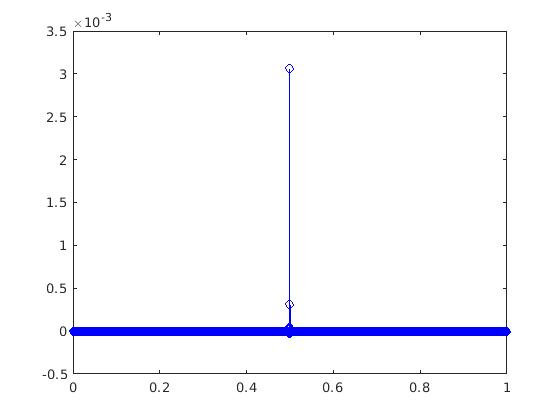
\includegraphics[width=1\linewidth]{images/lab2_18.jpg}
  \captionof{figure}{Improved ACF stemed (Blackman-Harris)}
\end{minipage}
\end{figure}

\newpage

\subsubsection{Triangular Window:}

Here we will get our filtered signal by triangle window. We get:

\begin{figure}[!hp]
    \begin{center}
      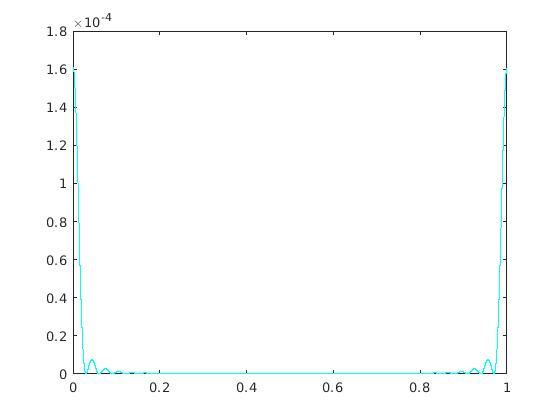
\includegraphics[width=0.6\textwidth]{images/lab2_26.jpg}
      \captionof{figure}{Improved PSD}
    \end{center}
\end{figure}

\begin{figure}[!hp]
\centering
\begin{minipage}{.5\textwidth}
  \centering
  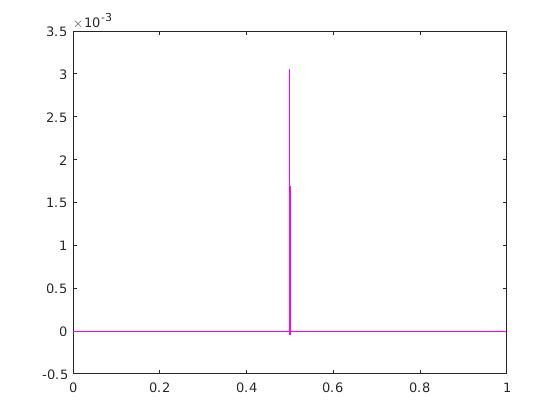
\includegraphics[width=1\linewidth]{images/lab2_22.jpg}
  \captionof{figure}{Improved ACF plotted (Bartlett)}
\end{minipage}%
\begin{minipage}{.5\textwidth}
  \centering
  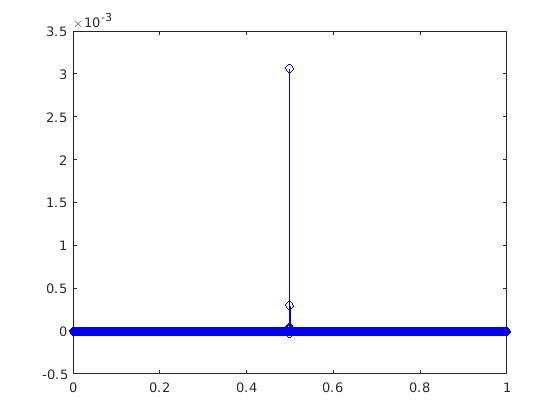
\includegraphics[width=1\linewidth]{images/lab2_23.jpg}
  \captionof{figure}{Improved ACF stemed (Bartlett)}
\end{minipage}
\end{figure}

\newpage

\begin{figure}[!hp]
\centering
\begin{minipage}{.5\textwidth}
  \centering
  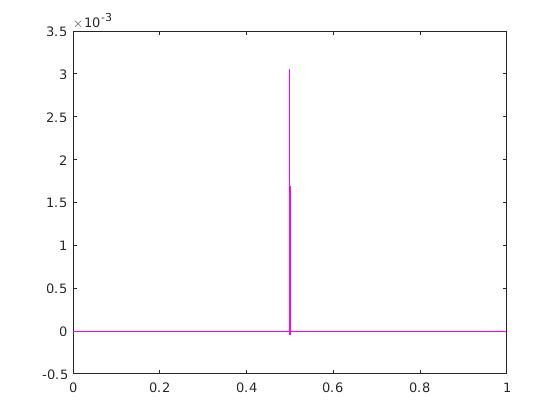
\includegraphics[width=1\linewidth]{images/lab2_24.jpg}
  \captionof{figure}{Improved ACF plotted (Blackman-Harris)}
\end{minipage}%
\begin{minipage}{.5\textwidth}
  \centering
  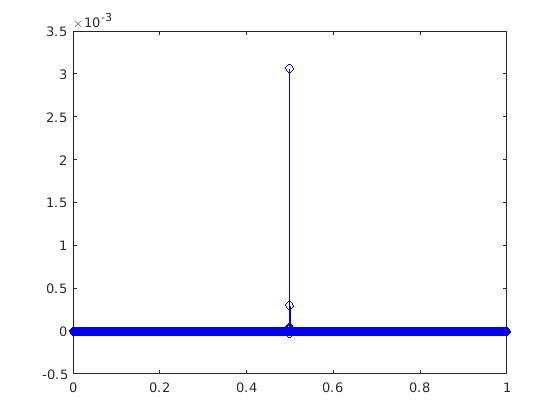
\includegraphics[width=1\linewidth]{images/lab2_25.jpg}
  \captionof{figure}{Improved ACF stemed (Blackman-Harris)}
\end{minipage}
\end{figure}

\subsubsection{Hamming Window:}

Here we will get our filtered signal by the Hamming window. Here are the results:

\begin{figure}[!hp]
    \begin{center}
      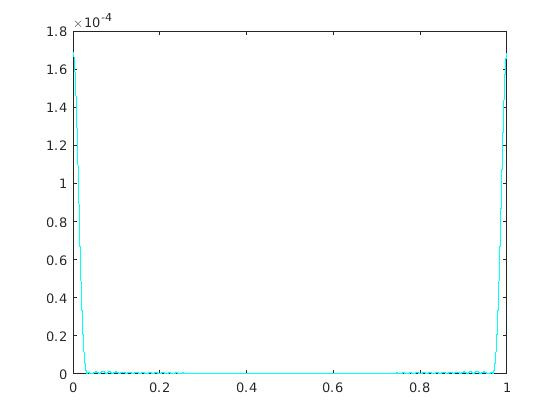
\includegraphics[width=0.6\textwidth]{images/lab2_33.jpg}
      \captionof{figure}{Improved PSD}
    \end{center}
\end{figure}

\newpage

\begin{figure}[!hp]
\centering
\begin{minipage}{.5\textwidth}
  \centering
  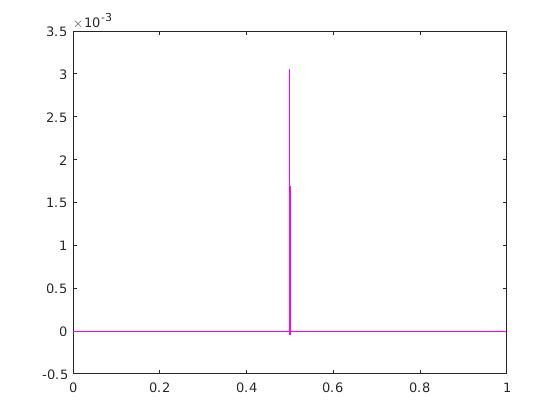
\includegraphics[width=1\linewidth]{images/lab2_29.jpg}
  \captionof{figure}{Improved ACF plotted (Bartlett)}
\end{minipage}%
\begin{minipage}{.5\textwidth}
  \centering
  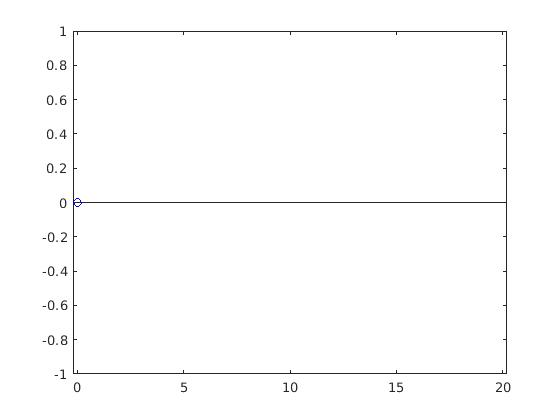
\includegraphics[width=1\linewidth]{images/lab2_30.jpg}
  \captionof{figure}{Improved ACF stemed (Bartlett)}
\end{minipage}
\end{figure}

\begin{figure}[!hp]
\centering
\begin{minipage}{.5\textwidth}
  \centering
  \includegraphics[width=1\linewidth]{images/lab2_31.jpg}
  \captionof{figure}{Improved ACF plotted (Blackman-Harris)}
\end{minipage}%
\begin{minipage}{.5\textwidth}
  \centering
  \includegraphics[width=1\linewidth]{images/lab2_32.jpg}
  \captionof{figure}{Improved ACF stemed (Blackman-Harris)}
\end{minipage}
\end{figure}

\newpage

\subsubsection{Bartlett Window:}

Here we will get our filtered signal by the Bartlett rectangular window. We get:

\begin{figure}[!hp]
    \begin{center}
      \includegraphics[width=0.6\textwidth]{images/lab2_40.jpg}
      \captionof{figure}{Improved PSD}
    \end{center}
\end{figure}

\begin{figure}[!hp]
\centering
\begin{minipage}{.5\textwidth}
  \centering
  \includegraphics[width=1\linewidth]{images/lab2_36.jpg}
  \captionof{figure}{Improved ACF plotted (Bartlett)}
\end{minipage}%
\begin{minipage}{.5\textwidth}
  \centering
  \includegraphics[width=1\linewidth]{images/lab2_37.jpg}
  \captionof{figure}{Improved ACF stemed (Bartlett)}
\end{minipage}
\end{figure}

\newpage

\begin{figure}[!hp]
\centering
\begin{minipage}{.5\textwidth}
  \centering
  \includegraphics[width=1\linewidth]{images/lab2_38.jpg}
  \captionof{figure}{Improved ACF plotted (Blackman-Harris)}
\end{minipage}%
\begin{minipage}{.5\textwidth}
  \centering
  \includegraphics[width=1\linewidth]{images/lab2_39.jpg}
  \captionof{figure}{Improved ACF stemed (Blackman-Harris)}
\end{minipage}
\end{figure}

\subsubsection{Blackman-Harris Window:}

Here we will get our filtered signal by the Blackman-Harris window. Here are the results:

\begin{figure}[!hp]
    \begin{center}
      \includegraphics[width=0.6\textwidth]{images/lab2_47.jpg}
      \captionof{figure}{Improved PSD}
    \end{center}
\end{figure}

\newpage

\begin{figure}[!hp]
\centering
\begin{minipage}{.5\textwidth}
  \centering
  \includegraphics[width=1\linewidth]{images/lab2_43.jpg}
  \captionof{figure}{Improved ACF plotted (Bartlett)}
\end{minipage}%
\begin{minipage}{.5\textwidth}
  \centering
  \includegraphics[width=1\linewidth]{images/lab2_44.jpg}
  \captionof{figure}{Improved ACF stemed (Bartlett)}
\end{minipage}
\end{figure}

\begin{figure}[!hp]
\centering
\begin{minipage}{.5\textwidth}
  \centering
  \includegraphics[width=1\linewidth]{images/lab2_45.jpg}
  \captionof{figure}{Improved ACF plotted (Blackman-Harris)}
\end{minipage}%
\begin{minipage}{.5\textwidth}
  \centering
  \includegraphics[width=1\linewidth]{images/lab2_46.jpg}
  \captionof{figure}{Improved ACF stemed (Blackman-Harris)}
\end{minipage}
\end{figure}

\newpage

\subsection{Improved Estimates: Low-degree filter:}

Let's move on to the low-degree filter. As before, for this section we will take the estimations done during the first study
with the first degree Butterworth filter.

We have the following PSD:

\begin{figure}[!hp]
    \begin{center}
      \includegraphics[width=0.6\textwidth]{images/lab2_54.jpg}
      \captionof{figure}{Estimated PSD}
    \end{center}
\end{figure}

If we estimate by the Bartlett method, we get the following ACF:

\begin{figure}[!hp]
\centering
\begin{minipage}{.5\textwidth}
  \centering
  \includegraphics[width=1\linewidth]{images/lab2_50.jpg}
  \captionof{figure}{Estimated by Bartlett ACF plotted}
\end{minipage}%
\begin{minipage}{.5\textwidth}
  \centering
  \includegraphics[width=1\linewidth]{images/lab2_51.jpg}
  \captionof{figure}{Estimated by Bartlett ACF stemed}
\end{minipage}
\end{figure}

\newpage

If we estimate by the Blackman-Harris method, we get the following ACF:

\begin{figure}[!hp]
\centering
\begin{minipage}{.5\textwidth}
  \centering
  \includegraphics[width=1\linewidth]{images/lab2_52.jpg}
  \captionof{figure}{Estimated by Blackman-Harris ACF plotted}
\end{minipage}%
\begin{minipage}{.5\textwidth}
  \centering
  \includegraphics[width=1\linewidth]{images/lab2_53.jpg}
  \captionof{figure}{Estimated by Blackman-Harris ACF stemed}
\end{minipage}
\end{figure}

\subsubsection{Rectangular Window:}

Here we will get our filtered signal by a filter which is our rectangular window. There are the results:

\begin{figure}[!hp]
    \begin{center}
      \includegraphics[width=0.6\textwidth]{images/lab2_61.jpg}
      \captionof{figure}{Improved PSD}
    \end{center}
\end{figure}

\newpage

\begin{figure}[!hp]
\centering
\begin{minipage}{.5\textwidth}
  \centering
  \includegraphics[width=1\linewidth]{images/lab2_57.jpg}
  \captionof{figure}{Improved ACF plotted (Bartlett)}
\end{minipage}%
\begin{minipage}{.5\textwidth}
  \centering
  \includegraphics[width=1\linewidth]{images/lab2_58.jpg}
  \captionof{figure}{Improved ACF stemed (Bartlett)}
\end{minipage}
\end{figure}

\begin{figure}[!hp]
\centering
\begin{minipage}{.5\textwidth}
  \centering
  \includegraphics[width=1\linewidth]{images/lab2_59.jpg}
  \captionof{figure}{Improved ACF plotted (Blackman-Harris)}
\end{minipage}%
\begin{minipage}{.5\textwidth}
  \centering
  \includegraphics[width=1\linewidth]{images/lab2_60.jpg}
  \captionof{figure}{Improved ACF stemed (Blackman-Harris)}
\end{minipage}
\end{figure}

\newpage

\subsubsection{Triangular Window:}

Here we will get our filtered signal by triangle window. We get:

\begin{figure}[!hp]
    \begin{center}
      \includegraphics[width=0.6\textwidth]{images/lab2_68.jpg}
      \captionof{figure}{Improved PSD}
    \end{center}
\end{figure}

\begin{figure}[!hp]
\centering
\begin{minipage}{.5\textwidth}
  \centering
  \includegraphics[width=1\linewidth]{images/lab2_64.jpg}
  \captionof{figure}{Improved ACF plotted (Bartlett)}
\end{minipage}%
\begin{minipage}{.5\textwidth}
  \centering
  \includegraphics[width=1\linewidth]{images/lab2_65.jpg}
  \captionof{figure}{Improved ACF stemed (Bartlett)}
\end{minipage}
\end{figure}

\newpage

\begin{figure}[!hp]
\centering
\begin{minipage}{.5\textwidth}
  \centering
  \includegraphics[width=1\linewidth]{images/lab2_66.jpg}
  \captionof{figure}{Improved ACF plotted (Blackman-Harris)}
\end{minipage}%
\begin{minipage}{.5\textwidth}
  \centering
  \includegraphics[width=1\linewidth]{images/lab2_67.jpg}
  \captionof{figure}{Improved ACF stemed (Blackman-Harris)}
\end{minipage}
\end{figure}

\subsubsection{Hamming Window:}

Here we will get our filtered signal by the Hamming window. Here are the results:

\begin{figure}[!hp]
    \begin{center}
      \includegraphics[width=0.6\textwidth]{images/lab2_75.jpg}
      \captionof{figure}{Improved PSD}
    \end{center}
\end{figure}

\newpage

\begin{figure}[!hp]
\centering
\begin{minipage}{.5\textwidth}
  \centering
  \includegraphics[width=1\linewidth]{images/lab2_71.jpg}
  \captionof{figure}{Improved ACF plotted (Bartlett)}
\end{minipage}%
\begin{minipage}{.5\textwidth}
  \centering
  \includegraphics[width=1\linewidth]{images/lab2_72.jpg}
  \captionof{figure}{Improved ACF stemed (Bartlett)}
\end{minipage}
\end{figure}

\begin{figure}[!hp]
\centering
\begin{minipage}{.5\textwidth}
  \centering
  \includegraphics[width=1\linewidth]{images/lab2_73.jpg}
  \captionof{figure}{Improved ACF plotted (Blackman-Harris)}
\end{minipage}%
\begin{minipage}{.5\textwidth}
  \centering
  \includegraphics[width=1\linewidth]{images/lab2_74.jpg}
  \captionof{figure}{Improved ACF stemed (Blackman-Harris)}
\end{minipage}
\end{figure}

\newpage

\subsubsection{Bartlett Window:}

Here we will get our filtered signal by the Bartlett rectangular window. We get:

\begin{figure}[!hp]
    \begin{center}
      \includegraphics[width=0.6\textwidth]{images/lab2_82.jpg}
      \captionof{figure}{Improved PSD}
    \end{center}
\end{figure}

\begin{figure}[!hp]
\centering
\begin{minipage}{.5\textwidth}
  \centering
  \includegraphics[width=1\linewidth]{images/lab2_78.jpg}
  \captionof{figure}{Improved ACF plotted (Bartlett)}
\end{minipage}%
\begin{minipage}{.5\textwidth}
  \centering
  \includegraphics[width=1\linewidth]{images/lab2_79.jpg}
  \captionof{figure}{Improved ACF stemed (Bartlett)}
\end{minipage}
\end{figure}

\newpage

\begin{figure}[!hp]
\centering
\begin{minipage}{.5\textwidth}
  \centering
  \includegraphics[width=1\linewidth]{images/lab2_80.jpg}
  \captionof{figure}{Improved ACF plotted (Blackman-Harris)}
\end{minipage}%
\begin{minipage}{.5\textwidth}
  \centering
  \includegraphics[width=1\linewidth]{images/lab2_81.jpg}
  \captionof{figure}{Improved ACF stemed (Blackman-Harris)}
\end{minipage}
\end{figure}

\subsubsection{Blackman-Harris Window:}

Here we will get our filtered signal by the Blackman-Harris window. Here are the results:

\begin{figure}[!hp]
    \begin{center}
      \includegraphics[width=0.6\textwidth]{images/lab2_89.jpg}
      \captionof{figure}{Improved PSD}
    \end{center}
\end{figure}

\newpage

\begin{figure}[!hp]
\centering
\begin{minipage}{.5\textwidth}
  \centering
  \includegraphics[width=1\linewidth]{images/lab2_85.jpg}
  \captionof{figure}{Improved ACF plotted (Bartlett)}
\end{minipage}%
\begin{minipage}{.5\textwidth}
  \centering
  \includegraphics[width=1\linewidth]{images/lab2_86.jpg}
  \captionof{figure}{Improved ACF stemed (Bartlett)}
\end{minipage}
\end{figure}

\begin{figure}[!hp]
\centering
\begin{minipage}{.5\textwidth}
  \centering
  \includegraphics[width=1\linewidth]{images/lab2_87.jpg}
  \captionof{figure}{Improved ACF plotted (Blackman-Harris)}
\end{minipage}%
\begin{minipage}{.5\textwidth}
  \centering
  \includegraphics[width=1\linewidth]{images/lab2_88.jpg}
  \captionof{figure}{Improved ACF stemed (Blackman-Harris)}
\end{minipage}
\end{figure}

\newpage

\subsection{Final Conclusion:}

As we can see, it's easier to work with smoothed graphs, for we can see the features of each plot better and it's not a messy drawing.
It's like filtering the noise again.

Tha Blackman-Harris window was the most aggresive one, followed by the Hamming window. The other windows respect more the natural form of the plot.

\newpage

\section{Study 3:}

\subsection{Theoretical Background:}

We have the three following systems:

A squarer:

\begin{equation}
  Y[n] =X^2[n]
\end{equation}

A half-wave rectifier:

\begin{equation}
  Y[n] =
    \begin{cases}
        X[n],& n: X[n]>0,\\
        0,    & n: X[n] \leq 0,
    \end{cases}
\end{equation}

An AM-SC modulator:

\begin{equation}
  Y[n] =X[n]cos(\Omega_{0} n)
\end{equation}

As we can see, non of them is LTI, which means that the output might or might not be Gaussian, and which also means that the PSD does not follow the formula we normally use, but an specific formula for the kind of non-linearity that the system presents.

Therefore, we have three special formulas:

\begin{equation}
  r_Y(\tau) = 2r_X^2(\tau) + r_X^2(0)
\end{equation}

\begin{equation}
  r_Y(\tau) = \frac{r_X(0)}{2\pi} + \frac{r_X(\tau)}{4} + \frac{r_X^2(\tau)}{4\pi r_X(o)} + ...
\end{equation}

\begin{equation}
  r_Y(\tau) = \frac{A^2}{2}(C^2 + r_X(\tau))cos(2\pi f_c \tau)
\end{equation}

They belong respectively with each one of the transformations above.

Knowing the value of $R_x(\tau)$, and therefore the value of $r_x(\tau)$, we translate them to the frequency domain to have the PSD expressions:

\begin{equation}
  R_Y[\theta] = 4\theta_c\Lambda[\frac{\theta}{2\theta_c}]+4\theta_c^2\delta[\theta]
\end{equation}

\begin{equation}
 R_Y[\theta] = \frac{1}{4\pi}\Lambda[\frac{\theta}{2\theta_c}]+\frac{1}{4}rect[\frac{\theta} {2\theta_c}]
+\frac{\theta_c}{\pi}\delta[\theta]
\end{equation}

\begin{equation}
  R_Y[\theta] = \frac{1}{4}(rect[\frac{\theta+\Omega_{0}} {2\theta_c}]+rect[\frac{\theta-\Omega_{0}} {2\theta_c}])
\end{equation}

\newpage

As done in the previous studies, we will use input noise. We will get it through in ideal low-pass filter, having the following result:

\begin{figure}[!hp]
    \begin{center}
    \includegraphics[width=0.6\textwidth]{images/lab3_6.jpg}
    \captionof{figure}{Filtered Signal}
    \end{center}
\end{figure}

\newpage

\subsection{Theoretical Analysis:}

First we can start with the filtered signal's PSD. We use the funtions that we have already used in previous studies, resulting in a PSD for the filter signal with the following plot:

\begin{figure}[!hp]
    \begin{center}
    \includegraphics[width=0.6\textwidth]{images/lab1_15.jpg}
    \captionof{figure}{PSD of the filtered signal}
    \end{center}
\end{figure}

If we get the signal through the squarer, the resulting PSD is:

\begin{figure}[!hp]
    \begin{center}
    \includegraphics[width=0.6\textwidth]{images/lab3_7.jpg}
    \captionof{figure}{PSD of the signal through the squarer}
    \end{center}
\end{figure}

\newpage

The PSD that we get after applying the half-wave rectifier to the filtered signal is:

\begin{figure}[!hp]
    \begin{center}
    \includegraphics[width=0.6\textwidth]{images/lab3_8.jpg}
    \captionof{figure}{PSD of the signal through the half-wave rectifier}
    \end{center}
\end{figure}

Lastly, the PSD resulting from AM-SC modulating the signal is:

\begin{figure}[!hp]
    \begin{center}
    \includegraphics[width=0.6\textwidth]{images/lab3_9.jpg}
    \captionof{figure}{PSD of the signal through the AM-SC modulator}
    \end{center}
\end{figure}

\newpage

\subsection{Estimations:}

We can continue with the estimations the three non-linear systems.

If we get the signal through the squarer, the resulting PSD is:

\begin{figure}[!hp]
    \begin{center}
    \includegraphics[width=0.6\textwidth]{images/lab3_16.jpg}
    \captionof{figure}{PSD of the signal through the squarer}
    \end{center}
\end{figure}

\newpage

The PSD that we get after applying the half-wave rectifier to the filtered signal is:

\begin{figure}[!hp]
    \begin{center}
    \includegraphics[width=0.6\textwidth]{images/lab3_18.jpg}
    \captionof{figure}{PSD of the signal through the Half-Wave Rectifier}
    \end{center}
\end{figure}

Lastly, the PSD resulting from AM-SC modulating the signal is:

\begin{figure}[!hp]
    \begin{center}
    \includegraphics[width=0.6\textwidth]{images/lab3_20.jpg}
    \captionof{figure}{PSD of the signal through the AM-SC modulator}
    \end{center}
\end{figure}

\newpage

\subsection{Improved Estimations:}

Here we will smooth the precious plots as done in Study 2:

\subsubsection{Rectangular Window:}

First we have the squarer PSD:
\begin{figure}[!hp]
    \begin{center}
    \includegraphics[width=0.6\textwidth]{images/lab3_22.jpg}
    \captionof{figure}{Improved PSD of the signal through the squarer}
    \end{center}
\end{figure}

Then we have the half-wave rectifier PSD:

\begin{figure}[!hp]
    \begin{center}
    \includegraphics[width=0.6\textwidth]{images/lab3_32.jpg}
    \captionof{figure}{Improved PSD of the signal through the Half-Wave Rectifier}
    \end{center}
\end{figure}

\newpage

Lastly, we have the AM-SC modulator PSD:

\begin{figure}[!hp]
    \begin{center}
    \includegraphics[width=0.6\textwidth]{images/lab3_42.jpg}
    \captionof{figure}{Improved PSD of the signal through the AM-SC modulator}
    \end{center}
\end{figure}

\subsubsection{Triangular Window:}

First we have the squarer PSD:
\begin{figure}[!hp]
    \begin{center}
    \includegraphics[width=0.6\textwidth]{images/lab3_24.jpg}
    \captionof{figure}{Improved PSD of the signal through the squarer}
    \end{center}
\end{figure}

\newpage

Then we have the half-wave rectifier PSD:

\begin{figure}[!hp]
    \begin{center}
    \includegraphics[width=0.6\textwidth]{images/lab3_34.jpg}
    \captionof{figure}{Improved PSD of the signal through the Half-Wave Rectifier}
    \end{center}
\end{figure}

Lastly, we have the AM-SC modulator PSD:

\begin{figure}[!hp]
    \begin{center}
    \includegraphics[width=0.6\textwidth]{images/lab3_44.jpg}
    \captionof{figure}{Improved PSD of the signal through the AM-SC modulator}
    \end{center}
\end{figure}

\newpage

\subsubsection{Hamming Window:}

First we have the squarer PSD:
\begin{figure}[!hp]
    \begin{center}
    \includegraphics[width=0.6\textwidth]{images/lab3_26.jpg}
    \captionof{figure}{Improved PSD of the signal through the squarer}
    \end{center}
\end{figure}

Then we have the half-wave rectifier PSD:

\begin{figure}[!hp]
    \begin{center}
    \includegraphics[width=0.6\textwidth]{images/lab3_36.jpg}
    \captionof{figure}{Improved PSD of the signal through the Half-Wave Rectifier}
    \end{center}
\end{figure}

\newpage

Lastly, we have the AM-SC modulator PSD:

\begin{figure}[!hp]
    \begin{center}
    \includegraphics[width=0.6\textwidth]{images/lab3_46.jpg}
    \captionof{figure}{Improved PSD of the signal through the AM-SC modulator}
    \end{center}
\end{figure}

\subsubsection{Bartlett Window:}

First we have the squarer PSD:
\begin{figure}[!hp]
    \begin{center}
    \includegraphics[width=0.6\textwidth]{images/lab3_28.jpg}
    \captionof{figure}{Improved PSD of the signal through the squarer}
    \end{center}
\end{figure}

\newpage

Then we have the half-wave rectifier PSD:

\begin{figure}[!hp]
    \begin{center}
    \includegraphics[width=0.6\textwidth]{images/lab3_38.jpg}
    \captionof{figure}{Improved PSD of the signal through the Half-Wave Rectifier}
    \end{center}
\end{figure}

Lastly, we have the AM-SC modulator PSD:

\begin{figure}[!hp]
    \begin{center}
    \includegraphics[width=0.6\textwidth]{images/lab3_48.jpg}
    \captionof{figure}{Improved PSD of the signal through the AM-SC modulator}
    \end{center}
\end{figure}

\newpage

\subsubsection{Blackman-Harris Window:}

First we have the squarer PSD:
\begin{figure}[!hp]
    \begin{center}
    \includegraphics[width=0.6\textwidth]{images/lab3_30.jpg}
    \captionof{figure}{Improved PSD of the signal through the squarer}
    \end{center}
\end{figure}

Then we have the half-wave rectifier PSD:

\begin{figure}[!hp]
    \begin{center}
    \includegraphics[width=0.6\textwidth]{images/lab3_40.jpg}
    \captionof{figure}{Improved PSD of the signal through the Half-Wave Rectifier}
    \end{center}
\end{figure}

\newpage

Lastly, we have the AM-SC modulator PSD:

\begin{figure}[!hp]
    \begin{center}
    \includegraphics[width=0.6\textwidth]{images/lab3_50.jpg}
    \captionof{figure}{Improved PSD of the signal through the AM-SC modulator}
    \end{center}
\end{figure}

\newpage

\subsection{Historiograms:}

Here we have the historiogram of each one of our systems.

First, the historiogram of our signal Y:

\begin{figure}[!hp]
    \begin{center}
    \includegraphics[width=0.6\textwidth]{images/lab3_52.jpg}
    \captionof{figure}{Historiogram of the filtered signal}
    \end{center}
\end{figure}

If we get the signal through the squarer, the resulting Historiogram is:

\begin{figure}[!hp]
    \begin{center}
    \includegraphics[width=0.6\textwidth]{images/lab3_53.jpg}
    \captionof{figure}{Historiogram of the signal through the squarer}
    \end{center}
\end{figure}

\newpage

The Historiogram that we get after applying the half-wave rectifier to the filtered signal is:

\begin{figure}[!hp]
    \begin{center}
    \includegraphics[width=0.6\textwidth]{images/lab3_54.jpg}
    \captionof{figure}{Historiogram of the signal through the half-wave rectifier}
    \end{center}
\end{figure}

Lastly, the Historiogram resulting from AM-SC modulating the signal is:

\begin{figure}[!hp]
    \begin{center}
    \includegraphics[width=0.6\textwidth]{images/lab3_55.jpg}
    \captionof{figure}{Historiogram of the signal through the AM-SC Modulator}
    \end{center}
\end{figure}

\newpage

\subsection{Final Comparation:}

My conclusion is that the half-wave rectifier is not a WSS system, because the PSD doesn't exist. The other two are WSS because the PSD exists and the plots make sense.

\newpage

\section{Study 4:}

\subsection{Theoretical Background:}

We hace two special operations:

\begin{equation}
  Y[n] = X[n](-1)^n
\end{equation}

\begin{equation}
  Y[n] =
    \begin{cases}
        X[n],& n: odd,\\
        0,    & n: even\\
    \end{cases}
\end{equation}

These represent two ways in which signals can be manipulated. We will get our every-study low-pass filtered White Gaussian Noise through these systems, to see if they're still WSS and to analize what happends with the PSDs of the signals that are being manipulated in this way in our every-day life situations.

The signals resulting from those systems are:

\begin{figure}[!hp]
\centering
\begin{minipage}{.5\textwidth}
  \centering
  \includegraphics[width=1\linewidth]{images/lab4_13.jpg}
  \captionof{figure}{Signal resulting from the first system}
\end{minipage}%
\begin{minipage}{.5\textwidth}
  \centering
  \includegraphics[width=1\linewidth]{images/lab4_16.jpg}
  \captionof{figure}{Signal resulting from the second system}
\end{minipage}
\end{figure}

\newpage

We have to calculate the PSD from the ACF:

\begin{equation}
  r_Y[\theta] = E\{Y[n+\theta]Y[n]\}
\end{equation}

I will not describe all the intermediate steps calculated here, so the final PSD result after the Fourier transform is for the first alternating system:

\begin{equation}
  R_Y[\theta] = R_X[\theta-0.5]
\end{equation}

And for the second system:

\begin{equation}
  R_Y[\theta] = \frac{1}{4}(R_X[\theta-0.5] + R_X[\theta])
\end{equation}

\newpage

\subsection{Theoretical Analysis:}

First we will start showing the plots of the theoretical PSD. Here is the PSD of the signal put through the first system:

\begin{figure}[!hp]
    \begin{center}
    \includegraphics[width=0.6\textwidth]{images/lab4_8.jpg}
    \captionof{figure}{PSD of the signal through the first system}
    \end{center}
\end{figure}

And here we have the PSD of the signal after the second system:

\begin{figure}[!hp]
    \begin{center}
      \includegraphics[width=0.6\textwidth]{images/lab4_9.jpg}
      \captionof{figure}{PSD of the signal through the second system}
    \end{center}
\end{figure}

\newpage

\subsection{Estimations:}

We can continue with the estimations the two systems.

If we get the signal through the first system, the resulting PSD is:

\begin{figure}[!hp]
    \begin{center}
    \includegraphics[width=0.6\textwidth]{images/lab4_19.jpg}
    \captionof{figure}{PSD of the signal through the first system}
    \end{center}
\end{figure}

The PSD that we get after applying the second system to the filtered signal is:

\begin{figure}[!hp]
    \begin{center}
    \includegraphics[width=0.6\textwidth]{images/lab4_21.jpg}
    \captionof{figure}{PSD of the signal through the second system}
    \end{center}
\end{figure}

\newpage

\subsection{Improved Estimations:}

Here we will smooth the precious plots as done in Study 2:

\subsubsection{Rectangular Window:}

First we have the first system:

\begin{figure}[!hp]
    \begin{center}
    \includegraphics[width=0.6\textwidth]{images/lab4_23.jpg}
    \captionof{figure}{Improved PSD of the signal through the first system}
    \end{center}
\end{figure}

Then we have the second system:

\begin{figure}[!hp]
    \begin{center}
    \includegraphics[width=0.6\textwidth]{images/lab4_33.jpg}
    \captionof{figure}{Improved PSD of the signal through the second system}
    \end{center}
\end{figure}

\newpage

\subsubsection{Triangular Window:}

First we have the first system:

\begin{figure}[!hp]
    \begin{center}
    \includegraphics[width=0.6\textwidth]{images/lab4_25.jpg}
    \captionof{figure}{Improved PSD of the signal through the first system}
    \end{center}
\end{figure}

Then we have the second system:

\begin{figure}[!hp]
    \begin{center}
    \includegraphics[width=0.6\textwidth]{images/lab4_35.jpg}
    \captionof{figure}{Improved PSD of the signal through the second system}
    \end{center}
\end{figure}

\newpage

\subsubsection{Hamming Window:}

First we have the first system:

\begin{figure}[!hp]
    \begin{center}
    \includegraphics[width=0.6\textwidth]{images/lab4_27.jpg}
    \captionof{figure}{Improved PSD of the signal through the first system}
    \end{center}
\end{figure}

Then we have the second system:

\begin{figure}[!hp]
    \begin{center}
    \includegraphics[width=0.6\textwidth]{images/lab4_37.jpg}
    \captionof{figure}{Improved PSD of the signal through the second system}
    \end{center}
\end{figure}

\newpage

\subsubsection{Bartlett Window:}

First we have the first system:

\begin{figure}[!hp]
    \begin{center}
    \includegraphics[width=0.6\textwidth]{images/lab4_29.jpg}
    \captionof{figure}{Improved PSD of the signal through the first system}
    \end{center}
\end{figure}

Then we have the second system:

\begin{figure}[!hp]
    \begin{center}
    \includegraphics[width=0.6\textwidth]{images/lab4_39.jpg}
    \captionof{figure}{Improved PSD of the signal through the second system}
    \end{center}
\end{figure}

\newpage

\subsubsection{Blackman-Harris Window:}

First we have the first system:

\begin{figure}[!hp]
    \begin{center}
    \includegraphics[width=0.6\textwidth]{images/lab4_31.jpg}
    \captionof{figure}{Improved PSD of the signal through the first system}
    \end{center}
\end{figure}

Then we have the second system:

\begin{figure}[!hp]
    \begin{center}
    \includegraphics[width=0.6\textwidth]{images/lab4_41.jpg}
    \captionof{figure}{Improved PSD of the signal through the second system}
    \end{center}
\end{figure}

\newpage

\subsection{Final Comparation:}

Both systmes are relatively similar when it comes to plotting the PSD. If we don't smooth the graphics, the plots are caotic and hard to read, but after putting the through a window (I think the rectangular window is the best here) it's easier to see that the first system is a bit smoother than the second one, because there are less differences between the peaks. 

\vspace{4cm}

\end{document}
